%%%%%%%%%%%%%%%%%%%%%%%%%%%%%%%%%%%%%%%%%%%%%%%%%%%%%%%%%%%%%%%%%%%%%%%%%%%%%%%
% GNN Research Experiments Technical Report
% Graph Neural Networks for Video Anomaly Detection
%%%%%%%%%%%%%%%%%%%%%%%%%%%%%%%%%%%%%%%%%%%%%%%%%%%%%%%%%%%%%%%%%%%%%%%%%%%%%%%

\documentclass[10pt,a4paper]{report}

%------------------------------------------------------------------------------
% Packages
%------------------------------------------------------------------------------
\usepackage[utf8]{inputenc}
\usepackage[T1]{fontenc}
\usepackage{amsmath,amssymb,amsfonts}
\usepackage{mathtools}
\usepackage{bm}  % Bold math symbols
\usepackage{graphicx}
\usepackage{xcolor}
\usepackage{tikz}
\usepackage{pgfplots}
\pgfplotsset{compat=1.16}
\usepackage{booktabs}
\usepackage{longtable}
\usepackage{multirow}
\usepackage{array}
\usepackage{float}
\usepackage{caption}
\usepackage{subcaption}
\usepackage{listings}
\usepackage{hyperref}
\usepackage{geometry}
\usepackage{fancyhdr}
\usepackage{setspace}
\usepackage{enumitem}
\usepackage{tocloft}
\usepackage{adjustbox}

%------------------------------------------------------------------------------
% TikZ Libraries
%------------------------------------------------------------------------------
\usetikzlibrary{
    shapes.geometric,
    arrows.meta,
    positioning,
    decorations.pathreplacing,
    calc,
    fit,
    backgrounds,
    matrix,
    chains,
    patterns,
    shadows,
    trees,
    mindmap
}

%------------------------------------------------------------------------------
% Page Setup
%------------------------------------------------------------------------------
\geometry{
    left=1in,
    right=1in,
    top=1in,
    bottom=1in
}

\setstretch{0.95}
\setlength{\parskip}{0.3em}
\setlength{\itemsep}{0.1em}
\setlength{\topsep}{0.2em}

%------------------------------------------------------------------------------
% Header and Footer
%------------------------------------------------------------------------------
\pagestyle{fancy}
\fancyhf{}
\fancyhead[L]{\leftmark}
\fancyhead[R]{\thepage}
\renewcommand{\headrulewidth}{0.4pt}

%------------------------------------------------------------------------------
% Hyperref Setup
%------------------------------------------------------------------------------
\hypersetup{
    colorlinks=true,
    linkcolor=blue!70!black,
    citecolor=green!50!black,
    urlcolor=blue!70!black,
    pdftitle={GNN Research Experiments Technical Report},
    pdfauthor={Research Team},
    pdfsubject={Graph Neural Networks for Video Anomaly Detection}
}

%------------------------------------------------------------------------------
% Code Listing Style
%------------------------------------------------------------------------------
\definecolor{codegreen}{rgb}{0,0.6,0}
\definecolor{codegray}{rgb}{0.5,0.5,0.5}
\definecolor{codepurple}{rgb}{0.58,0,0.82}
\definecolor{backcolour}{rgb}{0.95,0.95,0.92}

\lstdefinestyle{pythonstyle}{
    backgroundcolor=\color{backcolour},
    commentstyle=\color{codegreen},
    keywordstyle=\color{blue},
    numberstyle=\tiny\color{codegray},
    stringstyle=\color{codepurple},
    basicstyle=\ttfamily\footnotesize,
    breakatwhitespace=false,
    breaklines=true,
    captionpos=b,
    keepspaces=true,
    numbers=left,
    numbersep=5pt,
    showspaces=false,
    showstringspaces=false,
    showtabs=false,
    tabsize=2,
    frame=single,
    framerule=0.5pt
}
\lstset{style=pythonstyle}

%------------------------------------------------------------------------------
% Custom Colors
%------------------------------------------------------------------------------
\definecolor{inputcolor}{RGB}{100,149,237}
\definecolor{gcncolor}{RGB}{60,179,113}
\definecolor{poolcolor}{RGB}{255,165,0}
\definecolor{fccolor}{RGB}{147,112,219}
\definecolor{outputcolor}{RGB}{220,20,60}
\definecolor{normalcolor}{RGB}{34,139,34}
\definecolor{anomalouscolor}{RGB}{178,34,34}

%------------------------------------------------------------------------------
% Custom Commands
%------------------------------------------------------------------------------
\newcommand{\R}{\mathbb{R}}
\newcommand{\N}{\mathbb{N}}
\newcommand{\mat}[1]{\mathbf{#1}}
\newcommand{\vect}[1]{\bm{#1}}
\newcommand{\norm}[1]{\left\|#1\right\|}
\newcommand{\abs}[1]{\left|#1\right|}

%------------------------------------------------------------------------------
% Title Information - Custom titlepage
%------------------------------------------------------------------------------
\title{
    \vspace{-1cm}
    \rule{\linewidth}{0.5mm} \\[0.4cm]
    {\Huge \bfseries Graph Neural Networks for\\Video Anomaly Detection}\\[0.3cm]
    {\Large A Comprehensive Technical Report}\\[0.2cm]
    \rule{\linewidth}{0.5mm}
}

\author{}

\date{}

%%%%%%%%%%%%%%%%%%%%%%%%%%%%%%%%%%%%%%%%%%%%%%%%%%%%%%%%%%%%%%%%%%%%%%%%%%%%%%%
% Document Begin
%%%%%%%%%%%%%%%%%%%%%%%%%%%%%%%%%%%%%%%%%%%%%%%%%%%%%%%%%%%%%%%%%%%%%%%%%%%%%%%
\begin{document}

%------------------------------------------------------------------------------
% Title Page
%------------------------------------------------------------------------------
\begin{titlepage}
    \thispagestyle{empty}
    
    \begin{center}
        \vspace*{1cm}
        
        {\huge \bfseries Graph Neural Networks for\\Video Anomaly Detection}\\
        
        \vspace*{1.75cm}
        
        {\large Mini Project report submitted for the partial fulfillment\\}
        {\large of the requirements for the degree of \\}
        
        \vspace*{1cm}
        
        {\it {\large Bachelor of Technology} \\
        {\large in\\}
        {\large Electronics and Communication Engineering \\}}
        
        \vfill
        
        \vspace*{0.5cm}
        
        {\large by}\\
        
        \vspace*{0.5cm}
        
        {\large \bfseries Saumilya Gupta - 23UEC618}
        
        \vspace*{1cm}
        
        {\large \bfseries Mentor \\}
        {\large Dr. Preety Singh }
        
        \vfill
        
        \vspace*{0.5cm}
        
        \includegraphics[width=0.3\textwidth]{figures/LNMIIT.jpg}\\
        
        \vspace{1cm}
        
        {\bfseries\large Department of Electronics and Communication Engineering \\}
        {\large The LNM Institute of Information Technology, Jaipur\\}
        
        \vspace*{1.0cm}
        
        {\large \today\\}
        
        \vfill
        
    \end{center}
\end{titlepage}

\pagebreak

\vspace*{\fill}
\begin{center}
    \thispagestyle{empty}
    {\large Copyright \copyright~The LNMIIT 2025\\}{\large All rights reserved.}
\end{center}
\vspace*{\fill}

%------------------------------------------------------------------------------
% Abstract
%------------------------------------------------------------------------------
\begin{abstract}
\noindent
This technical report describes a comprehensive analysis on how Dynamic Graph Neural Networks can be used for video anomaly detection in traffic surveillance situations. To address this problem, we design a Temporal Graph Neural Network (Temporal DGNN) that employs spatial GCNs on a sequence of per-frame graphs followed by temporal GRU modeling. In our experiments, we use the NiAD\_large\_graphs dataset, consisting of 1,176 video samples (842 for training, 128 for validation, 206 for test) originating from the NiAD (Night-time Accident Detection) dataset. The pipeline translates 30 frames of video data into graph objects using PyTorch Geometric, with a different number of nodes per frame determined by vehicle detection. Data augmentation (brightness, flip, spatial shift) is performed on the anomalous class in order to address issues of class imbalance. The Temporal DGNN reaches a test accuracy of \textbf{89.32\%} with an \textbf{AUC-ROC of 0.81}, showing effective learning of spatial-temporal patterns for anomaly detection. This report discusses the complete data pipeline from video processing to graph formation, mathematical foundations of GNNs, Temporal DGNN architecture, and experimental results.

\vspace{0.5cm}
\noindent\textbf{Keywords:} Graph Neural Networks, Video Anomaly Detection, Dynamic Graphs, Traffic Surveillance, Deep Learning, Temporal Modeling, PyTorch Geometric
\end{abstract}

\newpage

%------------------------------------------------------------------------------
% Table of Contents
%------------------------------------------------------------------------------
\tableofcontents
\newpage

%------------------------------------------------------------------------------
% List of Figures and Tables
%------------------------------------------------------------------------------
\listoffigures
\listoftables
\newpage

%------------------------------------------------------------------------------
% Chapters
%------------------------------------------------------------------------------
%%%%%%%%%%%%%%%%%%%%%%%%%%%%%%%%%%%%%%%%%%%%%%%%%%%%%%%%%%%%%%%%%%%%%%%%%%%%%%%
% Chapter 1: Introduction
%%%%%%%%%%%%%%%%%%%%%%%%%%%%%%%%%%%%%%%%%%%%%%%%%%%%%%%%%%%%%%%%%%%%%%%%%%%%%%%

\chapter{Introduction}
\label{ch:introduction}

\section{Research Problem}

Video Anomaly Detection in traffic surveillance plays a vital role in intelligent transportation systems, enabling automated identification of accidents, dangerous driving practices, and other safety-critical events. The traditional method of this problem involves frame-by-frame analysis using convolutional neural networks (CNNs), which do not always take into consideration the complicated spatial relationships between vehicles and their development in relation to passage of time.

Graph Neural Networks (GNNs) offer a promising alternative by modeling vehicle interactions as graphs, where:
\begin{itemize}
    \item \textbf{Nodes} represent individual vehicles detected in each frame
    \item \textbf{Edges} encode spatial relations between cars in terms of Euclidean distances
    \item \textbf{Node features} encode vehicle properties (centroid, bounding box, class, timestamp)
    \item \textbf{Graph structure} preserves interaction topology which can possibly show anomalies
\end{itemize}

This work proposes a \textbf{Temporal Graph Neural Network (Temporal DGNN)}, which involves spatial processing of per-frame graphs using spatial GCN layers, followed by temporal processing using a GRU model. A 30-frame video can be broken down into a set of 30 dynamic graphs, with every frame generating a graph consisting solely of the vehicles that appear in a particular frame---no padding, no constant-size matrices, no missing value management required.

\section{Dataset: NiAD\_large\_graphs}

Our experiments are done using the \textbf{NiAD\_large\_graphs} dataset, which has been obtained from the NiAD (Night-time Accident Detection) dataset and processed using a customized node-feature data pipeline. The pipeline converts 30-frame video sequences into PyTorch Geometric graph objects stored as \texttt{.pt} files.

\begin{table}[H]
\centering
\caption{NiAD\_large\_graphs Dataset Statistics}
\label{tab:dataset_stats}
\begin{tabular}{lccccc}
\toprule
\textbf{Split} & \textbf{Total} & \textbf{Normal} & \textbf{Anomalous} & \textbf{Frames} & \textbf{Augmented} \\
\midrule
Training & 842 & 638 & 204 & 30 (fixed) & Yes (Anomalous only) \\
Validation & 128 & 112 & 16 & 30 (fixed) & No \\
Test & 206 & 184 & 22 & 30 (fixed) & No \\
\midrule
\textbf{Total} & \textbf{1,176} & \textbf{934} & \textbf{242} & -- & -- \\
\bottomrule
\end{tabular}
\end{table}

Data augmentation (brightness, flip, spatial shift) is applied only to anomalous training samples, resulting in 4$\times$ augmentation (51 $\times$ 4 = 204 videos). The test set has 8.4:1 Normal:Anomalous ratio, motivating Focal Loss usage.

\section{Research Contributions}

This work adds: (1) A pipeline from video to graph sequences with node features, using detection from YOLOv8 and graph representation from PyG, (2) A Temporal DGNN model with spatial GCN layers and GRU temporal modeling, (3) Clean dynamic graph representation without padding or sentinel values, (4) Class imbalance techniques for data augmentation with Focal Loss, and (5) Comprehensive experimental evaluation achieving 89.32\% accuracy with AUC-ROC of 0.81.

\section{Report Organization}

This report is organized as follows:

\begin{description}
    \item[Chapter 2: Mathematical Background] Describes the mathematical bases for Graph Neural Networks, including graph representation, message passing, GCN formulation, and concepts of temporal modeling.
    
    \item[Chapter 3: Data Pipeline] Describes how data moves from a raw video feed through graph representation, including vehicle detection and tracking, graph creation, and the PyTorch Geometric data format.
    
    \item[Chapter 4: Temporal DGNN Model] Description of the model structure involves spatial GCN layers, GRU temporal modeling, Focal Loss function, and training setup.
    
    \item[Chapter 5: Experiments and Results] Discusses experiments and their results in a comprehensive manner.
    
    \item[Chapter 6: Conclusion] Summarizes findings and discusses future research directions.
\end{description}

\section{System Architecture Overview}

Figure~\ref{fig:system_architecture} provides a high-level overview of the complete research system, from input videos to anomaly predictions.

\begin{figure}[H]
    \centering
    % System Architecture Diagram
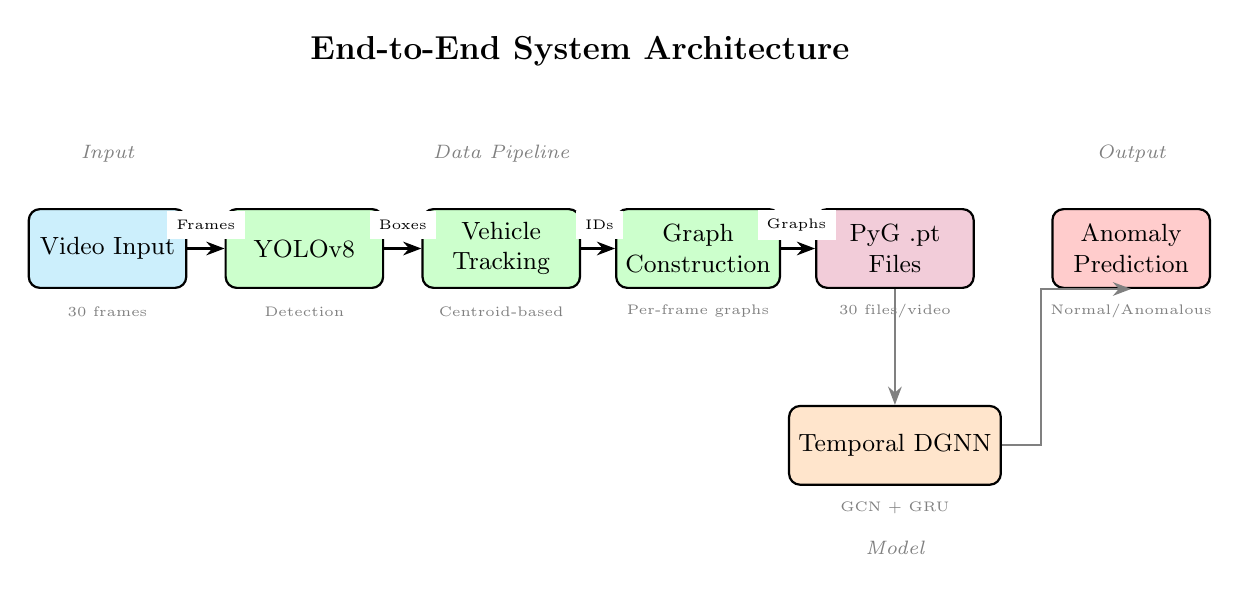
\begin{tikzpicture}[
    node distance=0.8cm and 1.2cm,
    box/.style={
        rectangle,
        rounded corners=4pt,
        minimum width=2cm,
        minimum height=1cm,
        align=center,
        draw=black,
        thick,
        font=\small
    },
    input/.style={box, fill=cyan!20},
    process/.style={box, fill=green!20},
    model/.style={box, fill=orange!20},
    output/.style={box, fill=red!20},
    data/.style={box, fill=purple!20},
    arrow/.style={-Stealth, thick},
    labeltext/.style={font=\tiny, gray}
]

% Title
\node[font=\large\bfseries] at (6, 5.5) {End-to-End System Architecture};

% Input Stage
\node[input] (video) at (0, 3) {Video Input};
\node[labeltext] at (0, 2.2) {30 frames};

% Detection Stage
\node[process] (yolo) at (2.5, 3) {YOLOv8};
\node[labeltext] at (2.5, 2.2) {Detection};

% Tracking Stage
\node[process] (tracking) at (5, 3) {Vehicle\\Tracking};
\node[labeltext] at (5, 2.2) {Centroid-based};

% Graph Construction
\node[process] (graph) at (7.5, 3) {Graph\\Construction};
\node[labeltext] at (7.5, 2.2) {Per-frame graphs};

% Storage
\node[data] (storage) at (10, 3) {PyG .pt\\Files};
\node[labeltext] at (10, 2.2) {30 files/video};

% Model
\node[model] (model) at (10, 0.5) {Temporal DGNN};
\node[labeltext] at (10, -0.3) {GCN + GRU};

% Output
\node[output] (output) at (13, 3) {Anomaly\\Prediction};
\node[labeltext] at (13, 2.2) {Normal/Anomalous};

% Arrows - Main flow
\draw[arrow] (video) -- (yolo);
\draw[arrow] (yolo) -- (tracking);
\draw[arrow] (tracking) -- (graph);
\draw[arrow] (graph) -- (storage);

% Model path
\draw[arrow, gray] (storage.south) -- (model.north);
\draw[arrow, gray] (model.east) -- ++(0.5, 0) |- (output.south);

% Flow labels
\node[font=\tiny, fill=white] at (1.25, 3.3) {Frames};
\node[font=\tiny, fill=white] at (3.75, 3.3) {Boxes};
\node[font=\tiny, fill=white] at (6.25, 3.3) {IDs};
\node[font=\tiny, fill=white] at (8.75, 3.3) {Graphs};

% Stage labels
\node[font=\scriptsize\itshape, gray] at (0, 4.2) {Input};
\node[font=\scriptsize\itshape, gray] at (5, 4.2) {Data Pipeline};
\node[font=\scriptsize\itshape, gray] at (10, -0.8) {Model};
\node[font=\scriptsize\itshape, gray] at (13, 4.2) {Output};

\end{tikzpicture}

    \caption{End-to-end system architecture for Temporal DGNN-based video anomaly detection. The pipeline processes surveillance videos through vehicle detection, tracking, and graph construction stages, producing 30 PyG graph files per video that are fed to the Temporal DGNN model for binary classification.}
    \label{fig:system_architecture}
\end{figure}

%%%%%%%%%%%%%%%%%%%%%%%%%%%%%%%%%%%%%%%%%%%%%%%%%%%%%%%%%%%%%%%%%%%%%%%%%%%%%%%
% Chapter 2: Mathematical Background
%%%%%%%%%%%%%%%%%%%%%%%%%%%%%%%%%%%%%%%%%%%%%%%%%%%%%%%%%%%%%%%%%%%%%%%%%%%%%%%

\chapter{Mathematical Background}
\label{ch:background}

This chapter presents the mathematical foundations of Graph Neural Networks required for understanding the models used in this research. We follow the notation and formulations from established literature \cite{kipf2017, kazemi2020, scarselli2008}.

\section{Graph Representation}

\subsection{Basic Definitions}

An \textbf{attributed graph} is represented as a tuple $G = (V, \mat{A}, \mat{X})$ where:

\begin{itemize}
    \item $V = \{v_1, v_2, \ldots, v_n\}$ is the set of vertices (nodes)
    \item $n = |V|$ denotes the number of nodes
    \item $\mat{A} \in \R^{n \times n}$ is the adjacency matrix
    \item $\mat{X} \in \R^{n \times d}$ is the feature matrix where $\mat{X}_i$ represents the $d$-dimensional features of node $v_i$
\end{itemize}

The adjacency matrix $\mat{A}$ encodes the graph structure:
\begin{equation}
    \mat{A}_{i,j} = \begin{cases}
        w_{ij} & \text{if there exists an edge between } v_i \text{ and } v_j \\
        0 & \text{otherwise}
    \end{cases}
\end{equation}

where $w_{ij} \in \R_+$ represents the edge weight.

\subsection{Graph Properties}

\textbf{Undirected graphs:} The adjacency matrix is symmetric, i.e., $\mat{A} = \mat{A}^\top$.

\textbf{Weighted graphs:} Edge weights can represent various properties such as:
\begin{itemize}
    \item \textbf{Distance:} Euclidean distance between nodes (as in our vehicle graphs)
    \item \textbf{Similarity:} Cosine similarity between node features
    \item \textbf{Connection strength:} Normalized affinity scores
\end{itemize}

In our application, each frame produces an \textbf{undirected weighted graph} where edge weights represent Euclidean distances between vehicle centroids.

\section{Message Passing Framework}

Graph Neural Networks operate through a \textbf{message passing} paradigm where node representations are iteratively updated by aggregating information from neighboring nodes.

\subsection{General Message Passing}

The general message passing framework consists of three operations at each layer $l$:

\begin{enumerate}
    \item \textbf{Message computation:} For each edge $(i, j)$, compute a message:
    \begin{equation}
        \vect{m}_{ij}^{(l)} = \phi^{(l)}\left(\vect{h}_i^{(l-1)}, \vect{h}_j^{(l-1)}, e_{ij}\right)
    \end{equation}
    
    \item \textbf{Aggregation:} Aggregate messages from all neighbors:
    \begin{equation}
        \vect{a}_i^{(l)} = \bigoplus_{j \in \mathcal{N}(i)} \vect{m}_{ij}^{(l)}
    \end{equation}
    where $\mathcal{N}(i)$ denotes the neighborhood of node $i$ and $\bigoplus$ is a permutation-invariant aggregation function (e.g., sum, mean, max).
    
    \item \textbf{Update:} Update node representation:
    \begin{equation}
        \vect{h}_i^{(l)} = \psi^{(l)}\left(\vect{h}_i^{(l-1)}, \vect{a}_i^{(l)}\right)
    \end{equation}
\end{enumerate}

Figure~\ref{fig:message_passing} illustrates the message passing process.

\begin{figure}[H]
    \centering
    % Message Passing Diagram
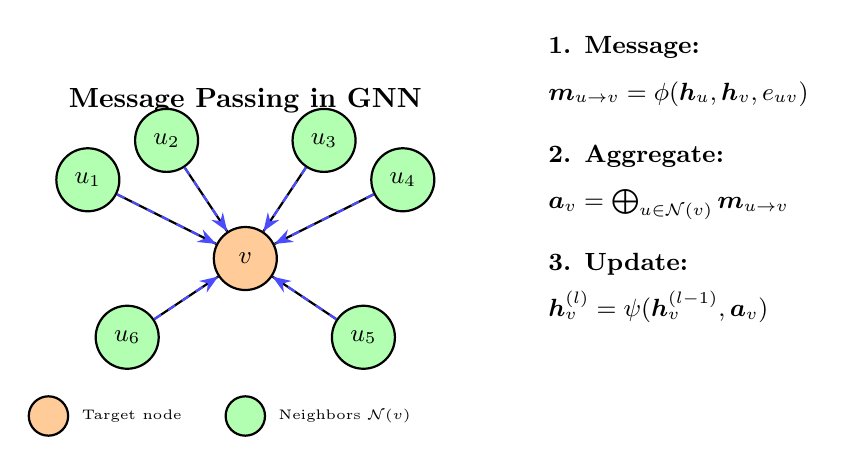
\begin{tikzpicture}[
    node distance=1.5cm,
    vertex/.style={
        circle,
        draw=black,
        thick,
        minimum size=0.8cm,
        font=\small
    },
    center/.style={vertex, fill=orange!40},
    neighbor/.style={vertex, fill=green!30},
    other/.style={vertex, fill=gray!20},
    arrow/.style={-Stealth, thick},
    messagearrow/.style={-Stealth, thick, blue!70, dashed}
]

% Title
\node[font=\bfseries] at (3, 3.5) {Message Passing in GNN};

% Center node
\node[center] (v) at (3, 1.5) {$v$};

% Neighbor nodes
\node[neighbor] (n1) at (1, 2.5) {$u_1$};
\node[neighbor] (n2) at (2, 3) {$u_2$};
\node[neighbor] (n3) at (4, 3) {$u_3$};
\node[neighbor] (n4) at (5, 2.5) {$u_4$};
\node[neighbor] (n5) at (4.5, 0.5) {$u_5$};
\node[neighbor] (n6) at (1.5, 0.5) {$u_6$};

% Edges
\draw[thick] (v) -- (n1);
\draw[thick] (v) -- (n2);
\draw[thick] (v) -- (n3);
\draw[thick] (v) -- (n4);
\draw[thick] (v) -- (n5);
\draw[thick] (v) -- (n6);

% Message arrows
\draw[messagearrow] (n1) -- (v);
\draw[messagearrow] (n2) -- (v);
\draw[messagearrow] (n3) -- (v);
\draw[messagearrow] (n4) -- (v);
\draw[messagearrow] (n5) -- (v);
\draw[messagearrow] (n6) -- (v);

% Equations
\node[align=left, font=\small] at (8.5, 2.5) {
    \textbf{1. Message:}\\[0.2cm]
    $\vect{m}_{u \to v} = \phi(\vect{h}_u, \vect{h}_v, e_{uv})$\\[0.4cm]
    \textbf{2. Aggregate:}\\[0.2cm]
    $\vect{a}_v = \bigoplus_{u \in \mathcal{N}(v)} \vect{m}_{u \to v}$\\[0.4cm]
    \textbf{3. Update:}\\[0.2cm]
    $\vect{h}_v^{(l)} = \psi(\vect{h}_v^{(l-1)}, \vect{a}_v)$
};

% Legend
\node[center, minimum size=0.5cm] at (0.5, -0.5) {};
\node[font=\tiny, right] at (0.8, -0.5) {Target node};
\node[neighbor, minimum size=0.5cm] at (3, -0.5) {};
\node[font=\tiny, right] at (3.3, -0.5) {Neighbors $\mathcal{N}(v)$};

\end{tikzpicture}





    \caption{Message passing in Graph Neural Networks. Each node aggregates features from its neighbors to update its representation.}
    \label{fig:message_passing}
\end{figure}

\section{Graph Convolutional Networks (GCN)}

The Graph Convolutional Network (GCN) \cite{kipf2017} is a specific instantiation of the message passing framework that has proven highly effective for graph-structured data.

\subsection{GCN Layer Formulation}

A single GCN layer transforms node features as follows:

\begin{equation}
\boxed{
    \mat{Z}^{(l)} = \sigma\left(\tilde{\mat{D}}^{-\frac{1}{2}} \tilde{\mat{A}} \tilde{\mat{D}}^{-\frac{1}{2}} \mat{Z}^{(l-1)} \mat{W}^{(l)}\right)
}
\label{eq:gcn_layer}
\end{equation}

where:
\begin{itemize}
    \item $\tilde{\mat{A}} = \mat{A} + \mat{I}_n$ is the adjacency matrix with added self-loops
    \item $\tilde{\mat{D}}$ is the degree matrix of $\tilde{\mat{A}}$ with $\tilde{\mat{D}}_{ii} = \sum_j \tilde{\mat{A}}_{ij}$
    \item $\mat{W}^{(l)} \in \R^{d_{l-1} \times d_l}$ is the learnable weight matrix for layer $l$
    \item $\sigma(\cdot)$ is a non-linear activation function (typically ReLU)
    \item $\mat{Z}^{(l-1)} \in \R^{n \times d_{l-1}}$ are the input node features
    \item $\mat{Z}^{(l)} \in \R^{n \times d_l}$ are the output node features
\end{itemize}

\subsection{Normalized Adjacency Matrix}

The symmetric normalization $\hat{\mat{A}} = \tilde{\mat{D}}^{-\frac{1}{2}} \tilde{\mat{A}} \tilde{\mat{D}}^{-\frac{1}{2}}$ ensures:

\begin{enumerate}
    \item \textbf{Eigenvalue bounds:} Eigenvalues are bounded in $[-1, 1]$
    \item \textbf{Numerical stability:} Prevents exploding/vanishing gradients
    \item \textbf{Scale invariance:} Feature aggregation is invariant to node degree
\end{enumerate}

The element-wise formula for the normalized adjacency is:
\begin{equation}
    \hat{\mat{A}}_{ij} = \frac{\tilde{\mat{A}}_{ij}}{\sqrt{\tilde{\mat{D}}_{ii}} \cdot \sqrt{\tilde{\mat{D}}_{jj}}}
\end{equation}

\subsection{Per-Node GCN Update}

For a single node $v_i$, the GCN update can be written as:
\begin{equation}
    \vect{h}_i^{(l)} = \sigma\left(\mat{W}^{(l)} \cdot \sum_{j \in \mathcal{N}(i) \cup \{i\}} \frac{1}{\sqrt{d_i + 1} \cdot \sqrt{d_j + 1}} \vect{h}_j^{(l-1)}\right)
\end{equation}

where $d_i$ and $d_j$ are the degrees of nodes $i$ and $j$ respectively.

Figure~\ref{fig:gcn_operation} illustrates the GCN convolution operation.

\begin{figure}[H]
    \centering
    % GCN Operation Diagram
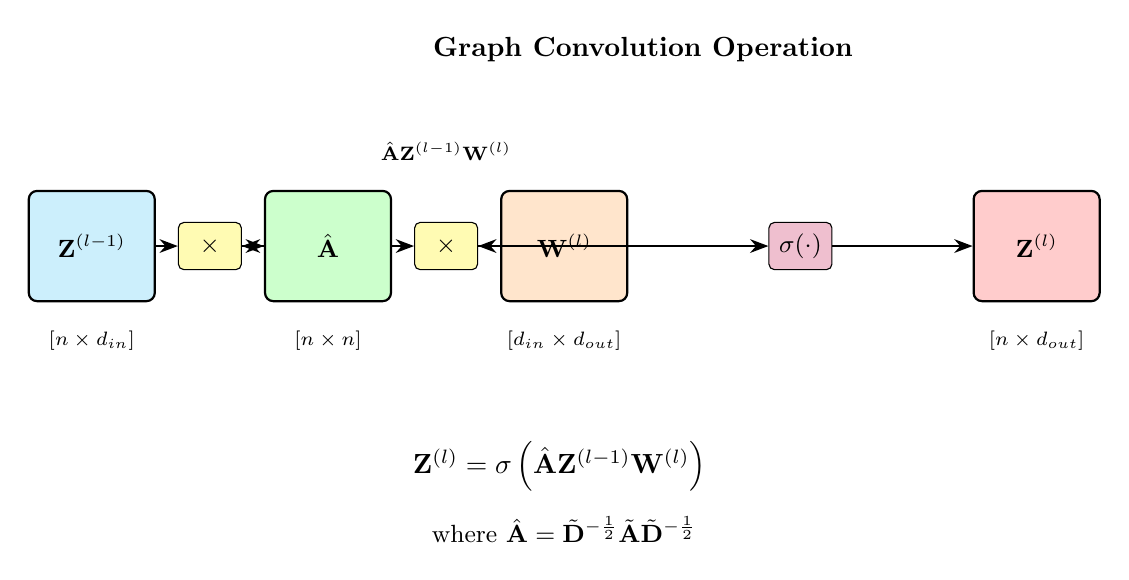
\begin{tikzpicture}[
    node distance=1.2cm,
    box/.style={
        rectangle,
        rounded corners=3pt,
        minimum width=1.6cm,
        minimum height=1.4cm,
        align=center,
        draw=black,
        thick,
        font=\small
    },
    opbox/.style={
        rectangle,
        rounded corners=2pt,
        minimum width=0.8cm,
        minimum height=0.6cm,
        align=center,
        draw=black,
        fill=yellow!30,
        font=\small
    },
    arrow/.style={-Stealth, thick}
]

% Title
\node[font=\bfseries] at (7, 4.5) {Graph Convolution Operation};

% Input features Z^(l-1)
\node[box, fill=cyan!20] (X) at (0, 2) {$\mat{Z}^{(l-1)}$};
\node[font=\scriptsize] at (0, 0.8) {$[n \times d_{in}]$};

% Adjacency A_hat
\node[box, fill=green!20] (A) at (3, 2) {$\hat{\mat{A}}$};
\node[font=\scriptsize] at (3, 0.8) {$[n \times n]$};

% Weight matrix W
\node[box, fill=orange!20] (W) at (6, 2) {$\mat{W}^{(l)}$};
\node[font=\scriptsize] at (6, 0.8) {$[d_{in} \times d_{out}]$};

% Output Z^(l)
\node[box, fill=red!20] (Z) at (12, 2) {$\mat{Z}^{(l)}$};
\node[font=\scriptsize] at (12, 0.8) {$[n \times d_{out}]$};

% Operators
\node[opbox] (mult1) at (1.5, 2) {$\times$};
\node[opbox] (mult2) at (4.5, 2) {$\times$};
\node[opbox, fill=purple!25] (sigma) at (9, 2) {$\sigma(\cdot)$};

% Arrows
\draw[arrow] (X) -- (mult1);
\draw[arrow] (A) -- (mult1);
\draw[arrow] (mult1) -- (A);
\draw[arrow] (A) -- (mult2);
\draw[arrow] (W) -- (mult2);
\draw[arrow] (mult2) -- (sigma);
\draw[arrow] (sigma) -- (Z);

% Intermediate labels
\node[font=\scriptsize, fill=white] at (4.5, 3.2) {$\hat{\mat{A}}\mat{Z}^{(l-1)}\mat{W}^{(l)}$};

% Equation
\node[font=\normalsize, align=center] at (6, -0.8) {
    $\mat{Z}^{(l)} = \sigma\left(\hat{\mat{A}} \mat{Z}^{(l-1)} \mat{W}^{(l)}\right)$
};
\node[font=\small] at (6, -1.6) {
    where $\hat{\mat{A}} = \tilde{\mat{D}}^{-\frac{1}{2}} \tilde{\mat{A}} \tilde{\mat{D}}^{-\frac{1}{2}}$
};

\end{tikzpicture}

    \caption{Graph Convolution operation. Node features are aggregated from neighbors with degree-normalized weights, then transformed through a learnable weight matrix.}
    \label{fig:gcn_operation}
\end{figure}

\section{Dynamic Graph Neural Networks}

Dynamic graphs extend static graphs by incorporating temporal evolution. Following \cite{kazemi2020}, we distinguish two types of dynamic graphs.

\subsection{Discrete-Time Dynamic Graphs (DTDG)}

A DTDG represents the graph as a sequence of snapshots:
\begin{equation}
    \mathcal{G} = \left[G^{(1)}, G^{(2)}, \ldots, G^{(T)}\right]
\end{equation}

where each $G^{(t)} = (V^{(t)}, \mat{A}^{(t)}, \mat{X}^{(t)})$ is a graph at time step $t$.

\textbf{Properties of DTDGs:}
\begin{itemize}
    \item Nodes may appear or disappear across time steps
    \item Edge structure may change between snapshots
    \item Node features may evolve over time
\end{itemize}

Our video anomaly detection problem naturally forms a DTDG where each frame corresponds to a time step.

\subsection{Continuous-Time Dynamic Graphs (CTDG)}

A CTDG represents the graph as a stream of timestamped events:
\begin{equation}
    \mathcal{G} = \{(u_i, v_i, t_i, \vect{e}_i)\}_{i=1}^{N}
\end{equation}

where each event represents an interaction between nodes $u_i$ and $v_i$ at time $t_i$ with optional features $\vect{e}_i$.

Figure~\ref{fig:dynamic_graph_types} illustrates both dynamic graph representations.

\begin{figure}[H]
    \centering
    % Dynamic Graph Types Diagram
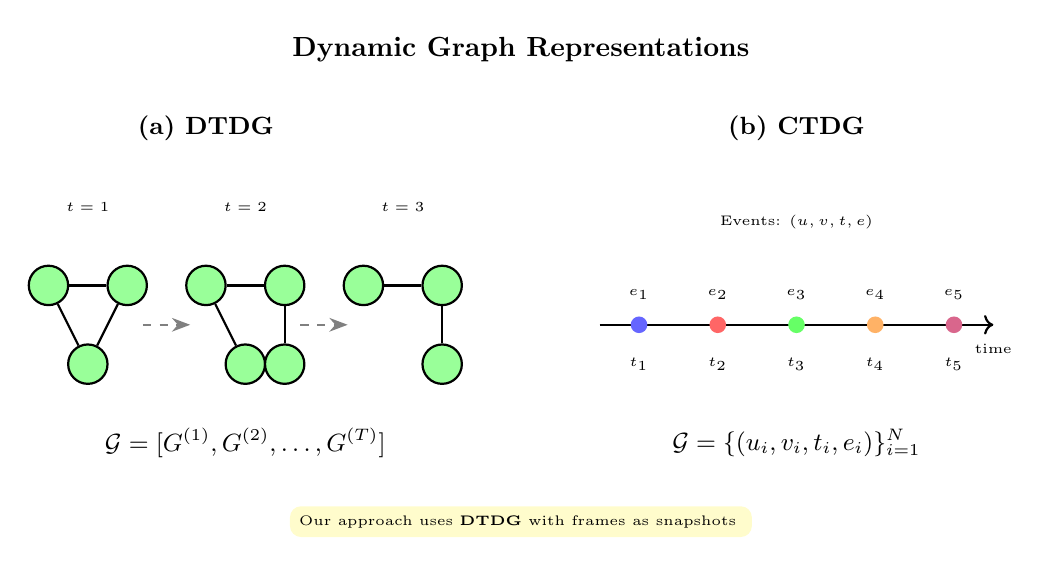
\begin{tikzpicture}[
    node distance=0.6cm,
    vertex/.style={
        circle,
        draw=black,
        thick,
        minimum size=0.5cm,
        font=\tiny
    },
    present/.style={vertex, fill=green!40},
    absent/.style={vertex, fill=gray!20, dashed},
    arrow/.style={-Stealth, thick}
]

% Title
\node[font=\bfseries] at (6, 5.5) {Dynamic Graph Representations};

% ===== DTDG Section =====
\node[font=\small\bfseries] at (2, 4.5) {(a) DTDG};

% Time labels
\node[font=\tiny] at (0.5, 3.5) {$t=1$};
\node[font=\tiny] at (2.5, 3.5) {$t=2$};
\node[font=\tiny] at (4.5, 3.5) {$t=3$};

% Snapshot 1
\node[present] (a1) at (0, 2.5) {};
\node[present] (b1) at (1, 2.5) {};
\node[present] (c1) at (0.5, 1.5) {};
\draw[thick] (a1) -- (b1);
\draw[thick] (a1) -- (c1);
\draw[thick] (b1) -- (c1);

% Snapshot 2
\node[present] (a2) at (2, 2.5) {};
\node[present] (b2) at (3, 2.5) {};
\node[present] (c2) at (2.5, 1.5) {};
\node[present] (d2) at (3, 1.5) {};
\draw[thick] (a2) -- (b2);
\draw[thick] (a2) -- (c2);
\draw[thick] (b2) -- (d2);
\draw[thick] (c2) -- (d2);

% Snapshot 3
\node[present] (a3) at (4, 2.5) {};
\node[present] (b3) at (5, 2.5) {};
\node[present] (d3) at (5, 1.5) {};
\draw[thick] (a3) -- (b3);
\draw[thick] (b3) -- (d3);

% Arrows between snapshots
\draw[arrow, gray, dashed] (1.2, 2) -- (1.8, 2);
\draw[arrow, gray, dashed] (3.2, 2) -- (3.8, 2);

% DTDG equation
\node[font=\small] at (2.5, 0.5) {$\mathcal{G} = [G^{(1)}, G^{(2)}, \ldots, G^{(T)}]$};

% ===== CTDG Section =====
\node[font=\small\bfseries] at (9.5, 4.5) {(b) CTDG};

% Timeline
\draw[thick, ->] (7, 2) -- (12, 2);
\node[font=\tiny] at (12, 1.7) {time};

% Events
\fill[blue!60] (7.5, 2) circle (3pt);
\node[font=\tiny, above] at (7.5, 2.2) {$e_1$};
\node[font=\tiny, below] at (7.5, 1.7) {$t_1$};

\fill[red!60] (8.5, 2) circle (3pt);
\node[font=\tiny, above] at (8.5, 2.2) {$e_2$};
\node[font=\tiny, below] at (8.5, 1.7) {$t_2$};

\fill[green!60] (9.5, 2) circle (3pt);
\node[font=\tiny, above] at (9.5, 2.2) {$e_3$};
\node[font=\tiny, below] at (9.5, 1.7) {$t_3$};

\fill[orange!60] (10.5, 2) circle (3pt);
\node[font=\tiny, above] at (10.5, 2.2) {$e_4$};
\node[font=\tiny, below] at (10.5, 1.7) {$t_4$};

\fill[purple!60] (11.5, 2) circle (3pt);
\node[font=\tiny, above] at (11.5, 2.2) {$e_5$};
\node[font=\tiny, below] at (11.5, 1.7) {$t_5$};

% Event descriptions
\node[font=\tiny, align=left] at (9.5, 3.3) {Events: $(u, v, t, e)$};

% CTDG equation
\node[font=\small] at (9.5, 0.5) {$\mathcal{G} = \{(u_i, v_i, t_i, e_i)\}_{i=1}^{N}$};

% Comparison note
\node[font=\tiny, align=center, fill=yellow!20, rounded corners] at (6, -0.5) {
    Our approach uses \textbf{DTDG} with frames as snapshots
};

\end{tikzpicture}

    \caption{Dynamic graph representations: (a) Discrete-Time Dynamic Graph (DTDG) as a sequence of snapshots, (b) Continuous-Time Dynamic Graph (CTDG) as a stream of events.}
    \label{fig:dynamic_graph_types}
\end{figure}

\section{Temporal Modeling with Recurrent Networks}

For processing temporal sequences of graph embeddings, we employ recurrent neural networks, specifically Gated Recurrent Units (GRU) \cite{cho2014}.

\subsection{GRU Formulation}

The GRU updates hidden states using gating mechanisms:

\begin{align}
    \vect{z}_t &= \sigma\left(\mat{W}_z \vect{x}_t + \mat{U}_z \vect{h}_{t-1} + \vect{b}_z\right) & \text{(Update gate)} \\
    \vect{r}_t &= \sigma\left(\mat{W}_r \vect{x}_t + \mat{U}_r \vect{h}_{t-1} + \vect{b}_r\right) & \text{(Reset gate)} \\
    \tilde{\vect{h}}_t &= \tanh\left(\mat{W}_h \vect{x}_t + \mat{U}_h (\vect{r}_t \odot \vect{h}_{t-1}) + \vect{b}_h\right) & \text{(Candidate)} \\
    \vect{h}_t &= (1 - \vect{z}_t) \odot \vect{h}_{t-1} + \vect{z}_t \odot \tilde{\vect{h}}_t & \text{(Output)}
\end{align}

where $\odot$ denotes element-wise multiplication.

\subsection{Combining GCN with GRU}

For dynamic graphs, we combine spatial (GCN) and temporal (GRU) processing:

\begin{enumerate}
    \item \textbf{Spatial encoding:} Apply GCN layers to each snapshot $G^{(t)}$:
    \begin{equation}
        \mat{H}^{(t)} = \text{GCN}\left(G^{(t)}\right) \in \R^{n \times d}
    \end{equation}
    
    \item \textbf{Graph-level pooling:} Aggregate node features to graph-level:
    \begin{equation}
        \vect{g}^{(t)} = \text{POOL}\left(\mat{H}^{(t)}\right) \in \R^{d}
    \end{equation}
    
    \item \textbf{Temporal encoding:} Process sequence with GRU:
    \begin{equation}
        \vect{o} = \text{GRU}\left(\left[\vect{g}^{(1)}, \vect{g}^{(2)}, \ldots, \vect{g}^{(T)}\right]\right)
    \end{equation}
\end{enumerate}

\section{Graph Pooling Operations}

Graph pooling aggregates node features: Mean Pool $\vect{g} = \frac{1}{|V|} \sum_{v \in V} \vect{h}_v$, Max Pool $\vect{g} = \max_{v \in V} \vect{h}_v$, or Sum Pool $\vect{g} = \sum_{v \in V} \vect{h}_v$. Our model uses mean pooling.

\section{Focal Loss for Class Imbalance}

For handling class imbalance in binary classification, we employ Focal Loss \cite{lin2017}.

\subsection{Focal Loss Formulation}

The Focal Loss is defined as:
\begin{equation}
\boxed{
    \text{FL}(p_t) = -\alpha_t (1 - p_t)^\gamma \log(p_t)
}
\label{eq:focal_loss}
\end{equation}

where:
\begin{itemize}
    \item $p_t$ is the predicted probability for the true class
    \item $\gamma \geq 0$ is the focusing parameter
    \item $\alpha_t \in [0, 1]$ is the class balancing factor
\end{itemize}

\subsection{Class Balancing Factor}

The balancing factor $\alpha$ is computed from the training set distribution:
\begin{equation}
    \alpha = \frac{N_{\text{normal}}}{N_{\text{normal}} + N_{\text{anomalous}}}
\end{equation}

For a sample with label $y$:
\begin{equation}
    \alpha_t = \begin{cases}
        \alpha & \text{if } y = 0 \text{ (Normal)} \\
        1 - \alpha & \text{if } y = 1 \text{ (Anomalous)}
    \end{cases}
\end{equation}

\subsection{Focusing Effect}

The modulating factor $(1 - p_t)^\gamma$ has the following properties:
\begin{itemize}
    \item When $p_t \to 1$ (well-classified): $(1 - p_t)^\gamma \to 0$, reducing loss contribution
    \item When $p_t \to 0$ (misclassified): $(1 - p_t)^\gamma \to 1$, maintaining full loss
\end{itemize}

This causes the model to focus on hard-to-classify examples while down-weighting easy examples.

\section{Summary of Mathematical Notation}

Table~\ref{tab:notation} summarizes the mathematical notation used throughout this report.

\begin{table}[H]
\centering
\caption{Summary of Mathematical Notation}
\label{tab:notation}
\begin{tabular}{cl}
\toprule
\textbf{Symbol} & \textbf{Description} \\
\midrule
$G = (V, \mat{A}, \mat{X})$ & Attributed graph \\
$V$ & Set of vertices (nodes) \\
$n = |V|$ & Number of nodes \\
$\mat{A} \in \R^{n \times n}$ & Adjacency matrix \\
$\mat{X} \in \R^{n \times d}$ & Node feature matrix \\
$\mat{W}^{(l)}$ & Weight matrix for layer $l$ \\
$\mat{Z}^{(l)}$ & Node embeddings at layer $l$ \\
$\vect{h}_i$ & Feature vector of node $i$ \\
$\mathcal{N}(i)$ & Neighborhood of node $i$ \\
$\tilde{\mat{A}}$ & Adjacency with self-loops ($\mat{A} + \mat{I}$) \\
$\tilde{\mat{D}}$ & Degree matrix of $\tilde{\mat{A}}$ \\
$\sigma(\cdot)$ & Activation function \\
$\odot$ & Element-wise (Hadamard) product \\
$T$ & Number of time steps \\
$\gamma$ & Focal loss focusing parameter \\
$\alpha$ & Focal loss balancing factor \\
\bottomrule
\end{tabular}
\end{table}





%%%%%%%%%%%%%%%%%%%%%%%%%%%%%%%%%%%%%%%%%%%%%%%%%%%%%%%%%%%%%%%%%%%%%%%%%%%%%%%
% Chapter 3: Data Pipeline
%%%%%%%%%%%%%%%%%%%%%%%%%%%%%%%%%%%%%%%%%%%%%%%%%%%%%%%%%%%%%%%%%%%%%%%%%%%%%%%

\chapter{Data Pipeline}
\label{ch:data_pipeline}

This chapter details the node-feature-based data processing pipeline that converts raw surveillance videos into dynamic graph sequences suitable for the Temporal DGNN model. The pipeline is implemented in Python and leverages YOLOv8 for vehicle detection and PyTorch Geometric for graph representation.

\section{Pipeline Overview}

The data pipeline consists of five main stages:

\begin{enumerate}
    \item \textbf{Video Discovery:} Scan input directory for video files organized by split and class
    \item \textbf{Vehicle Detection:} Apply YOLOv8 to detect vehicles in each frame
    \item \textbf{Vehicle Tracking:} Assign consistent IDs to vehicles across frames
    \item \textbf{Graph Construction:} Build per-frame PyG graphs with dynamic node counts
    \item \textbf{Data Storage:} Save graphs as \texttt{.pt} files (30 per video) with CSV manifests
\end{enumerate}

Figure~\ref{fig:pipeline_flow} illustrates the complete pipeline flow.

\begin{figure}[H]
    \centering
    % Pipeline Flow Diagram
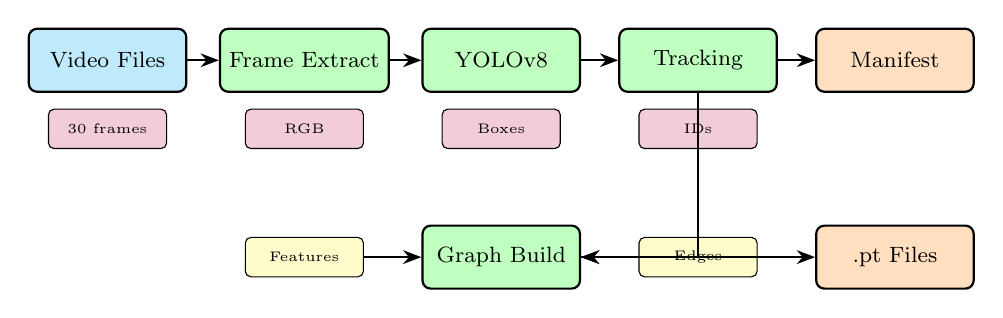
\begin{tikzpicture}[
    node distance=0.6cm and 1cm,
    box/.style={
        rectangle,
        rounded corners=3pt,
        minimum width=2cm,
        minimum height=0.8cm,
        align=center,
        draw=black,
        thick,
        font=\footnotesize
    },
    smallbox/.style={
        rectangle,
        rounded corners=2pt,
        minimum width=1.5cm,
        minimum height=0.5cm,
        align=center,
        draw=black,
        font=\tiny
    },
    input/.style={box, fill=cyan!25},
    process/.style={box, fill=green!25},
    output/.style={box, fill=orange!25},
    data/.style={smallbox, fill=purple!20},
    arrow/.style={-Stealth, thick}
]

% Stage 1: Input
\node[input] (video) at (0, 2.5) {Video Files};
\node[data, below=0.2cm of video] (d1) {30 frames};

% Stage 2: Frame Extraction
\node[process] (frames) at (2.5, 2.5) {Frame Extract};
\node[data, below=0.2cm of frames] (d2) {RGB};

% Stage 3: YOLO Detection
\node[process] (yolo) at (5, 2.5) {YOLOv8};
\node[data, below=0.2cm of yolo] (d3) {Boxes};

% Stage 4: Vehicle Tracking
\node[process] (track) at (7.5, 2.5) {Tracking};
\node[data, below=0.2cm of track] (d4) {IDs};

% Stage 5: Graph Construction
\node[process] (graph) at (5, 0) {Graph Build};

% Sub-processes
\node[smallbox, fill=yellow!20] (nodes) at (2.5, 0) {Features};
\node[smallbox, fill=yellow!20] (edges) at (7.5, 0) {Edges};

% Stage 6: Output
\node[output] (pt) at (10, 0) {.pt Files};
\node[output] (csv) at (10, 2.5) {Manifest};

% Arrows - main flow
\draw[arrow] (video) -- (frames);
\draw[arrow] (frames) -- (yolo);
\draw[arrow] (yolo) -- (track);
\draw[arrow] (track) -- (csv);
\draw[arrow] (track) |- (graph);

% Arrows - graph construction
\draw[arrow] (nodes) -- (graph);
\draw[arrow] (edges) -- (graph);
\draw[arrow] (graph) -- (pt);

\end{tikzpicture}

    \caption{Data pipeline flowchart showing the transformation from raw video to PyTorch Geometric graph sequence.}
    \label{fig:pipeline_flow}
\end{figure}

\section{Video Processing}

Videos are organized by split (Training/Validation/Testing) and class (Normal/Accident). Each video is processed to extract exactly 30 frames using YOLOv8 with confidence threshold 0.3 for vehicle classes 2, 3, 5, 7 (car, motorcycle, bus, truck).

\section{Vehicle Detection}

\subsection{YOLO Configuration}

We use YOLOv8 (nano variant) for efficient vehicle detection:

\begin{table}[H]
\centering
\caption{YOLO Detection Configuration}
\label{tab:yolo_config}
\begin{tabular}{ll}
\toprule
\textbf{Parameter} & \textbf{Value} \\
\midrule
Model & YOLOv8n (nano) \\
Confidence Threshold & 0.3 \\
Vehicle Classes & 2 (car), 3 (motorcycle), 5 (bus), 7 (truck) \\
Device & CUDA GPU \\
\bottomrule
\end{tabular}
\end{table}

YOLO outputs bounding boxes, centroids, class IDs, and confidence scores for each detected vehicle.


\section{Vehicle Tracking}

Centroid-based tracking maintains consistent vehicle IDs across frames using distance matching (max\_distance=100 pixels, max\_disappeared=10 frames). The Hungarian algorithm matches detections to existing tracks.


\section{Graph Construction}

\subsection{Dynamic Graph Representation}

Unlike fixed-size matrix approaches, each frame produces a graph containing \textbf{only the vehicles present in that frame}. This eliminates padding and missing value handling:

\begin{itemize}
    \item \textbf{Node Features:} $\mat{X}_t \in \R^{N_t \times 8}$ where $N_t$ is the number of vehicles in frame $t$
    \item \textbf{Edge Index:} Sparse representation of fully-connected graph
    \item \textbf{Edge Weight:} Euclidean distance between centroids
    \item \textbf{Node IDs:} Tracking IDs for temporal consistency
\end{itemize}

\subsection{Node Features (8 dimensions)}

Each node (vehicle) has 8 features:

\begin{table}[H]
\centering
\caption{Node Feature Specification}
\label{tab:node_features}
\begin{tabular}{clll}
\toprule
\textbf{Index} & \textbf{Feature} & \textbf{Description} & \textbf{Range} \\
\midrule
0 & centroid\_x & X-coordinate of bounding box center & $[0, \text{width}]$ \\
1 & centroid\_y & Y-coordinate of bounding box center & $[0, \text{height}]$ \\
2 & bbox\_x & Top-left X coordinate & $[0, \text{width}]$ \\
3 & bbox\_y & Top-left Y coordinate & $[0, \text{height}]$ \\
4 & bbox\_w & Bounding box width & $[0, \text{width}]$ \\
5 & bbox\_h & Bounding box height & $[0, \text{height}]$ \\
6 & class\_id & YOLO class ID & $\{2, 3, 5, 7\}$ \\
7 & timestamp & Normalized time: frame\_index / 29 & $[0, 1]$ \\
\bottomrule
\end{tabular}
\end{table}



\subsection{Edge Construction}

Edges connect all pairs of vehicles in each frame with weights based on Euclidean distance:

\begin{equation}
    \text{edge\_weight}_{ij} = \|\vect{c}_i - \vect{c}_j\|_2 = \sqrt{(c_{x,i} - c_{x,j})^2 + (c_{y,i} - c_{y,j})^2}
\end{equation}

For a frame with $N_t$ nodes, the fully connected graph has $N_t \times (N_t - 1)$ directed edges.

Figure~\ref{fig:graph_construction} illustrates the graph construction process.

\begin{figure}[H]
    \centering
    % Graph Construction Diagram
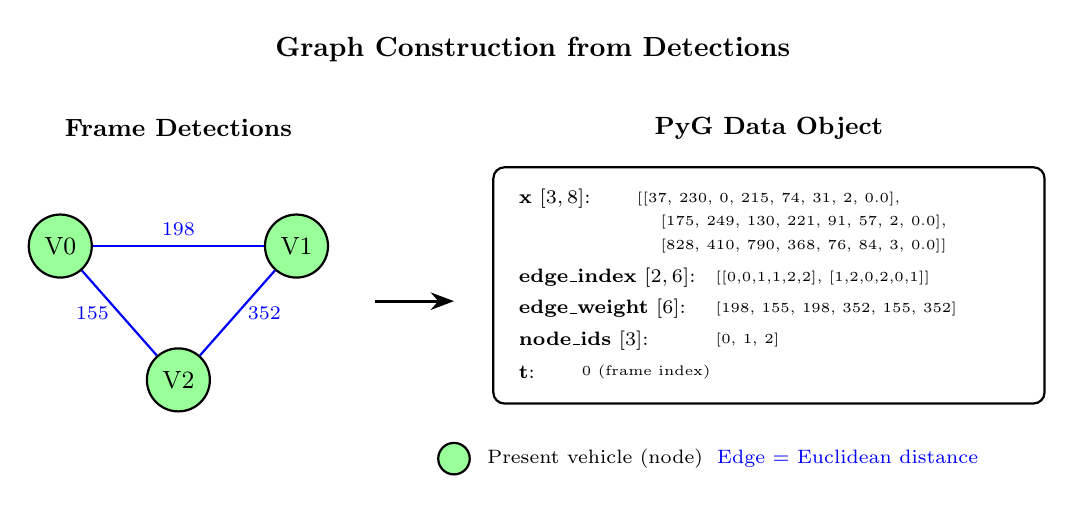
\begin{tikzpicture}[
    node distance=1cm,
    vertex/.style={
        circle,
        draw=black,
        thick,
        minimum size=0.8cm,
        font=\small,
        align=center
    },
    present/.style={vertex, fill=green!40},
    arrow/.style={-Stealth, thick}
]

% Title
\node[font=\bfseries] at (6, 5) {Graph Construction from Detections};

% Left side: Detections
\node[font=\small\bfseries] at (1.5, 4) {Frame Detections};

% Detected vehicles (only present ones)
\node[present] (v0) at (0, 2.5) {V0};
\node[present] (v1) at (3, 2.5) {V1};
\node[present] (v2) at (1.5, 0.8) {V2};

% Edges with distances
\draw[thick, blue] (v0) -- node[above, font=\scriptsize] {198} (v1);
\draw[thick, blue] (v0) -- node[left, font=\scriptsize] {155} (v2);
\draw[thick, blue] (v1) -- node[right, font=\scriptsize] {352} (v2);

% Arrow
\draw[arrow, very thick] (4, 1.8) -- (5, 1.8);

% Right side: PyG Data
\node[font=\small\bfseries] at (9, 4) {PyG Data Object};

% Data box
\draw[thick, rounded corners] (5.5, 0.5) rectangle (12.5, 3.5);

% x: node features
\node[font=\scriptsize, anchor=west] at (5.7, 3.1) {\textbf{x} $[3, 8]$:};
\node[font=\tiny, anchor=west] at (7.2, 3.1) {[[37, 230, 0, 215, 74, 31, 2, 0.0],};
\node[font=\tiny, anchor=west] at (7.5, 2.8) {[175, 249, 130, 221, 91, 57, 2, 0.0],};
\node[font=\tiny, anchor=west] at (7.5, 2.5) {[828, 410, 790, 368, 76, 84, 3, 0.0]]};

% edge_index
\node[font=\scriptsize, anchor=west] at (5.7, 2.1) {\textbf{edge\_index} $[2, 6]$:};
\node[font=\tiny, anchor=west] at (8.2, 2.1) {[[0,0,1,1,2,2], [1,2,0,2,0,1]]};

% edge_weight
\node[font=\scriptsize, anchor=west] at (5.7, 1.7) {\textbf{edge\_weight} $[6]$:};
\node[font=\tiny, anchor=west] at (8.2, 1.7) {[198, 155, 198, 352, 155, 352]};

% node_ids
\node[font=\scriptsize, anchor=west] at (5.7, 1.3) {\textbf{node\_ids} $[3]$:};
\node[font=\tiny, anchor=west] at (8.2, 1.3) {[0, 1, 2]};

% t
\node[font=\scriptsize, anchor=west] at (5.7, 0.9) {\textbf{t}:};
\node[font=\tiny, anchor=west] at (6.5, 0.9) {0 (frame index)};

% Legend
\node[present, minimum size=0.4cm] at (5, -0.2) {};
\node[font=\scriptsize, right] at (5.3, -0.2) {Present vehicle (node)};
\node[font=\scriptsize, blue] at (10, -0.2) {Edge = Euclidean distance};

\end{tikzpicture}

    \caption{Graph construction from vehicle detections. Nodes represent present vehicles only, edges represent spatial distances.}
    \label{fig:graph_construction}
\end{figure}


\section{PyTorch Geometric Data Format}

Each frame graph is stored as a PyTorch Geometric \texttt{Data} object with fields: \texttt{x} (node features [N, 8]), \texttt{edge\_index} ([2, E]), \texttt{edge\_weight} ([E]), \texttt{node\_ids} ([N]), and \texttt{t} (frame index).

Each video produces 30 \texttt{.pt} files organized by split and class. CSV manifests track video metadata (path, label, vehicle counts).

Figure~\ref{fig:hdf5_structure} illustrates the file structure.

\begin{figure}[H]
    \centering
    % PyG File Structure Diagram
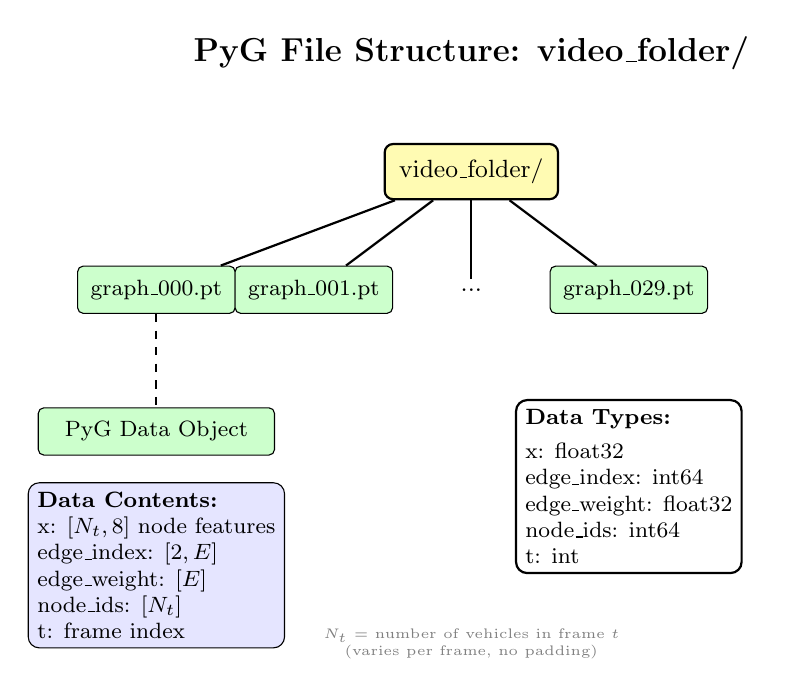
\begin{tikzpicture}[
    folder/.style={
        rectangle,
        rounded corners=3pt,
        draw=black,
        thick,
        fill=yellow!30,
        font=\small,
        minimum height=0.7cm,
        minimum width=2.2cm,
        align=center
    },
    file/.style={
        rectangle,
        rounded corners=2pt,
        draw=black,
        fill=green!20,
        font=\footnotesize,
        minimum height=0.6cm,
        minimum width=2cm,
        align=center
    },
    arrow/.style={draw, thick, -}
]

% Title
\node[font=\bfseries\large] at (4, 3) {PyG File Structure: video\_folder/};

% Root
\node[folder] (root) at (4, 1.5) {video\_folder/};

% Graph files
\node[file] (g0) at (0, 0) {graph\_000.pt};
\node[file] (g1) at (2, 0) {graph\_001.pt};
\node[font=\small] (dots) at (4, 0) {...};
\node[file] (g29) at (6, 0) {graph\_029.pt};

% Connect root to files
\draw[arrow] (root) -- (g0);
\draw[arrow] (root) -- (g1);
\draw[arrow] (root) -- (dots);
\draw[arrow] (root) -- (g29);

% Expand one graph file
\node[file, minimum width=3cm] (data) at (0, -1.8) {PyG Data Object};

\draw[arrow, dashed] (g0) -- (data);

% Data object contents
\node[font=\footnotesize, align=left, fill=blue!10, draw, rounded corners] at (0, -3.5) {
    \textbf{Data Contents:}\\
    x: $[N_t, 8]$ node features\\
    edge\_index: $[2, E]$\\
    edge\_weight: $[E]$\\
    node\_ids: $[N_t]$\\
    t: frame index
};

% Data type annotations box
\node[font=\footnotesize, align=left, fill=white, draw, rounded corners, thick] at (6, -2.5) {
    \textbf{Data Types:}\\[0.1cm]
    x: float32\\
    edge\_index: int64\\
    edge\_weight: float32\\
    node\_ids: int64\\
    t: int
};

% Note about dynamic size
\node[font=\tiny, gray, align=center] at (4, -4.5) {$N_t$ = number of vehicles in frame $t$\\(varies per frame, no padding)};

\end{tikzpicture}

    \caption{PyTorch Geometric file structure. Each frame produces a separate \texttt{.pt} file containing the graph data object.}
    \label{fig:hdf5_structure}
\end{figure}

Graph sequences are loaded by iterating through 30 \texttt{.pt} files per video. The \texttt{node\_ids} field enables temporal alignment by sorting nodes by tracking IDs before processing.

\section{Data Augmentation}

Data augmentation is applied \textbf{only to anomalous training samples} to address class imbalance.

\subsection{Augmentation Strategies}

\begin{enumerate}
    \item \textbf{Original:} Unmodified video (no suffix)
    \item \textbf{Brightness:} Adjusted lighting conditions (suffix: \texttt{\_bright})
    \item \textbf{Horizontal Flip:} Mirror transformation (suffix: \texttt{\_flip})
    \item \textbf{Spatial Shift:} Left-shifted frames (suffix: \texttt{\_shift\_left})
\end{enumerate}

\subsection{Augmentation Statistics}

\begin{table}[H]
\centering
\caption{Training Set Augmentation Breakdown}
\label{tab:augmentation_stats}
\begin{tabular}{lccc}
\toprule
\textbf{Class} & \textbf{Original} & \textbf{Augmented} & \textbf{Total} \\
\midrule
Normal & 638 & 0 & 638 \\
Anomalous & 51 & 153 (3 variants each) & 204 \\
\midrule
\textbf{Total} & \textbf{689} & \textbf{153} & \textbf{842} \\
\bottomrule
\end{tabular}
\end{table}

Figure~\ref{fig:data_augmentation} visualizes the augmentation strategies.

\begin{figure}[H]
    \centering
    % Data Augmentation Diagram
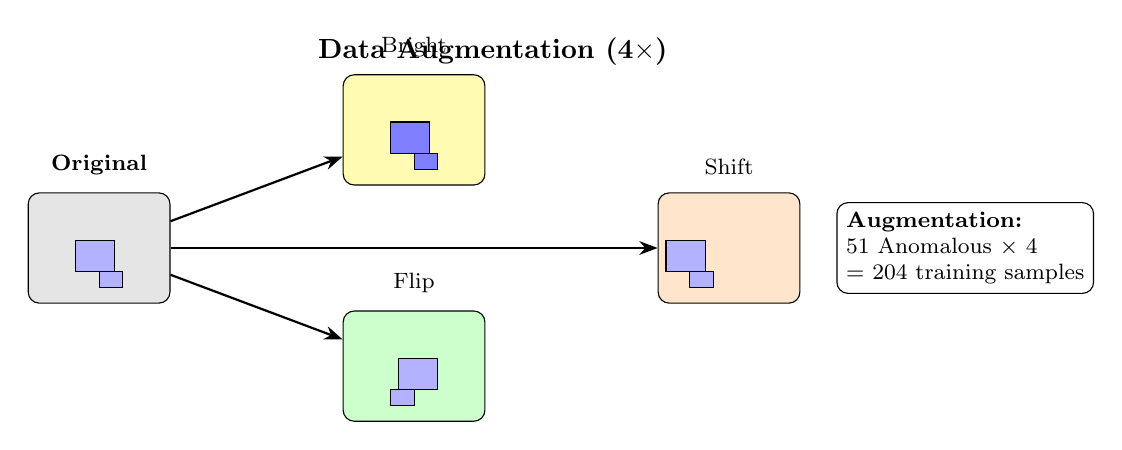
\begin{tikzpicture}[
    frame/.style={
        rectangle,
        draw=black,
        rounded corners,
        minimum width=1.8cm,
        minimum height=1.4cm,
        font=\tiny
    },
    arrow/.style={-Stealth, thick}
]

% Title
\node[font=\bfseries] at (5, 5) {Data Augmentation (4$\times$)};

% Original frame
\node[frame, fill=gray!20] (orig) at (0, 2.5) {};
\node[font=\footnotesize\bfseries, above=0.1cm of orig] {Original};
\draw[fill=blue!30, draw=black] (-0.3, 2.2) rectangle (0.2, 2.6);
\draw[fill=blue!30, draw=black] (0, 2.0) rectangle (0.3, 2.2);

% Brightness adjusted
\node[frame, fill=yellow!30] (bright) at (4, 4) {};
\node[font=\footnotesize, above=0.1cm of bright] {Bright};
\draw[fill=blue!50, draw=black] (3.7, 3.7) rectangle (4.2, 4.1);
\draw[fill=blue!50, draw=black] (4, 3.5) rectangle (4.3, 3.7);

% Horizontal flip
\node[frame, fill=green!20] (flip) at (4, 1) {};
\node[font=\footnotesize, above=0.1cm of flip] {Flip};
\draw[fill=blue!30, draw=black] (3.8, 0.7) rectangle (4.3, 1.1);
\draw[fill=blue!30, draw=black] (3.7, 0.5) rectangle (4, 0.7);

% Spatial shift
\node[frame, fill=orange!20] (shift) at (8, 2.5) {};
\node[font=\footnotesize, above=0.1cm of shift] {Shift};
\draw[fill=blue!30, draw=black] (7.2, 2.2) rectangle (7.7, 2.6);
\draw[fill=blue!30, draw=black] (7.5, 2.0) rectangle (7.8, 2.2);

% Arrows
\draw[arrow] (orig) -- (bright);
\draw[arrow] (orig) -- (flip);
\draw[arrow] (orig) -- (shift);

% Statistics box
\node[draw, rounded corners, fill=white, font=\footnotesize, align=left] at (11, 2.5) {
    \textbf{Augmentation:}\\
    51 Anomalous $\times$ 4\\
    = 204 training samples
};

\end{tikzpicture}

    \caption{Data augmentation strategies applied to anomalous training videos. Each original video generates 4 variants (including original) for class balancing.}
    \label{fig:data_augmentation}
\end{figure}


\section{Pipeline Summary}

\begin{table}[H]
\centering
\caption{Pipeline Processing Summary}
\label{tab:pipeline_summary}
\begin{tabular}{ll}
\toprule
\textbf{Metric} & \textbf{Value} \\
\midrule
Total videos processed & 1,176 \\
Training videos & 842 (638 Normal + 204 Anomalous) \\
Validation videos & 128 \\
Test videos & 206 \\
Frames per video & 30 (fixed) \\
Node features per vehicle & 8 \\
Vehicle classes detected & 4 (car, motorcycle, bus, truck) \\
YOLO confidence threshold & 0.3 \\
Storage format & PyTorch Geometric \texttt{.pt} files \\
Graph type & Fully connected (per frame) \\
\bottomrule
\end{tabular}
\end{table}

%%%%%%%%%%%%%%%%%%%%%%%%%%%%%%%%%%%%%%%%%%%%%%%%%%%%%%%%%%%%%%%%%%%%%%%%%%%%%%%
% Chapter 4: Temporal DGNN Model
%%%%%%%%%%%%%%%%%%%%%%%%%%%%%%%%%%%%%%%%%%%%%%%%%%%%%%%%%%%%%%%%%%%%%%%%%%%%%%%

\chapter{Temporal DGNN Model}
\label{ch:model_dynamic_gnn}

This chapter presents the Temporal Graph Neural Network (Temporal DGNN) model, which processes temporal sequences of graphs by combining spatial graph convolutions with temporal GRU modeling. This approach is evaluated on the NiAD\_large\_graphs dataset containing 1,176 videos.

\section{Model Overview}

The Temporal DGNN architecture follows a simple yet effective design:

\begin{enumerate}
    \item \textbf{Per-frame GCN processing:} Each frame's graph is processed independently by two GCN layers
    \item \textbf{Identity alignment:} Nodes are sorted by \texttt{node\_ids} for temporal consistency
    \item \textbf{Mean pooling:} Frame-level embeddings are computed via mean pooling
    \item \textbf{GRU temporal modeling:} Frame embeddings are processed sequentially by GRU
    \item \textbf{Classification:} Final hidden state is passed through a classifier
\end{enumerate}

\section{Architecture Components}

\subsection{Overall Architecture}

The model processes a list of 30 PyG graph objects and outputs a binary classification:

\begin{figure}[H]
    \centering
    % Dynamic GNN Architecture Diagram
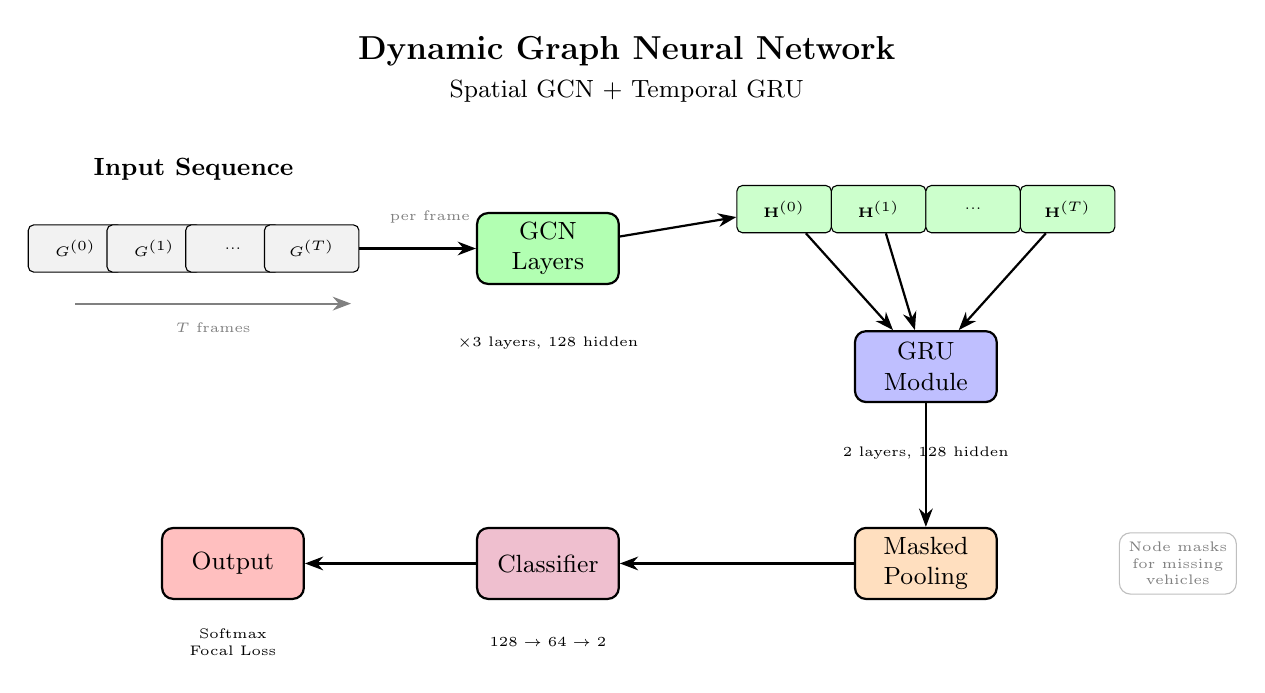
\begin{tikzpicture}[
    node distance=0.8cm and 1cm,
    box/.style={
        rectangle,
        rounded corners=4pt,
        minimum width=1.8cm,
        minimum height=0.9cm,
        align=center,
        draw=black,
        thick,
        font=\small
    },
    frame/.style={
        rectangle,
        rounded corners=2pt,
        minimum width=1.2cm,
        minimum height=0.6cm,
        draw=black,
        font=\tiny,
        fill=gray!10,
        align=center
    },
    input/.style={box, fill=cyan!25},
    gcn/.style={box, fill=green!30},
    temporal/.style={box, fill=blue!25},
    pool/.style={box, fill=orange!25},
    fc/.style={box, fill=purple!25},
    output/.style={box, fill=red!25},
    arrow/.style={thick, -Stealth}
]

% Title
\node[font=\large\bfseries] at (7, 7.5) {Dynamic Graph Neural Network};
\node[font=\small] at (7, 7) {Spatial GCN + Temporal GRU};

% Input frames
\node[font=\small\bfseries] at (1.5, 6) {Input Sequence};
\node[frame] (f0) at (0, 5) {$G^{(0)}$};
\node[frame] (f1) at (1, 5) {$G^{(1)}$};
\node[frame] (f2) at (2, 5) {...};
\node[frame] (fT) at (3, 5) {$G^{(T)}$};

% Per-frame GCN processing
\node[gcn] (gcn) at (6, 5) {GCN\\Layers};
\node[font=\tiny, align=center] at (6, 3.8) {$\times 3$ layers, 128 hidden};

% Per-frame outputs
\node[frame, fill=green!20] (h0) at (9, 5.5) {$\mat{H}^{(0)}$};
\node[frame, fill=green!20] (h1) at (10.2, 5.5) {$\mat{H}^{(1)}$};
\node[frame, fill=green!20] (h2) at (11.4, 5.5) {...};
\node[frame, fill=green!20] (hT) at (12.6, 5.5) {$\mat{H}^{(T)}$};

% Temporal module
\node[temporal] (gru) at (10.8, 3.5) {GRU\\Module};
\node[font=\tiny, align=center] at (10.8, 2.4) {2 layers, 128 hidden};

% Global pooling
\node[pool] (pool) at (10.8, 1) {Masked\\Pooling};

% Classifier
\node[fc] (fc) at (6, 1) {Classifier};
\node[font=\tiny] at (6, 0) {$128 \to 64 \to 2$};

% Output
\node[output] (output) at (2, 1) {Output};
\node[font=\tiny, align=center] at (2, 0) {Softmax\\Focal Loss};

% Arrows - input to GCN
\draw[arrow] (fT) -- (gcn);
\node[font=\tiny, gray, above] at (4.5, 5.2) {per frame};

% Arrows - GCN to frame outputs
\draw[arrow] (gcn) -- (h0);

% Arrows - outputs to GRU
\draw[arrow] (h0) -- (gru);
\draw[arrow] (h1) -- (gru);
\draw[arrow] (hT) -- (gru);

% Arrows - GRU to pooling to classifier
\draw[arrow] (gru) -- (pool);
\draw[arrow] (pool) -- (fc);
\draw[arrow] (fc) -- (output);

% Node masks annotation
\node[font=\tiny, gray, align=center, fill=white, draw=gray!50, rounded corners] at (14, 1) {
    Node masks\\for missing\\vehicles
};

% Time annotation
\draw[arrow, gray] (0, 4.3) -- (3.5, 4.3);
\node[font=\tiny, gray] at (1.75, 4) {$T$ frames};

\end{tikzpicture}

    \caption{Temporal DGNN architecture: per-frame GCN processing followed by GRU temporal modeling for video-level classification.}
    \label{fig:dynamic_gnn_architecture}
\end{figure}

The model architecture: GCNConv(8, 64) $\rightarrow$ GCNConv(64, 64) $\rightarrow$ mean pooling $\rightarrow$ GRU(64, 128) $\rightarrow$ Linear(128, 2). Nodes are sorted by \texttt{node\_ids} before processing to ensure temporal consistency.

\section{Model Configuration}

\subsection{Architecture Parameters}

\begin{table}[H]
\centering
\caption{Temporal DGNN Architecture Configuration}
\label{tab:temporal_gnn_config}
\begin{tabular}{ll}
\toprule
\textbf{Parameter} & \textbf{Value} \\
\midrule
\multicolumn{2}{l}{\textit{Input}} \\
Node feature dimension & 8 \\
Sequence length & 30 frames \\
\midrule
\multicolumn{2}{l}{\textit{GCN Layers}} \\
Number of GCN layers & 2 \\
Layer 1 & GCNConv(8, 64) \\
Layer 2 & GCNConv(64, 64) \\
Activation & ReLU \\
\midrule
\multicolumn{2}{l}{\textit{GRU Module}} \\
Input dimension & 64 \\
Hidden dimension & 128 \\
Number of layers & 1 \\
\midrule
\multicolumn{2}{l}{\textit{Classifier}} \\
Input dimension & 128 \\
Output dimension & 2 \\
\bottomrule
\end{tabular}
\end{table}

\subsection{Training Configuration}

\begin{table}[H]
\centering
\caption{Training Configuration (from config.yaml)}
\label{tab:training_config}
\begin{tabular}{ll}
\toprule
\textbf{Parameter} & \textbf{Value} \\
\midrule
\multicolumn{2}{l}{\textit{Optimization}} \\
Optimizer & Adam \\
Learning rate & $1 \times 10^{-3}$ \\
Weight decay & $1 \times 10^{-5}$ \\
Gradient clipping & 1.0 \\
\midrule
\multicolumn{2}{l}{\textit{Training}} \\
Batch size & 8 \\
Max epochs & 100 \\
GPU & cuda:4 \\
\midrule
\multicolumn{2}{l}{\textit{Scheduler}} \\
Type & ReduceLROnPlateau \\
Monitor & val\_loss \\
Mode & min \\
\midrule
\multicolumn{2}{l}{\textit{Early Stopping}} \\
Patience & 15 epochs \\
Min delta & 0.0001 \\
\midrule
\multicolumn{2}{l}{\textit{Checkpointing}} \\
Save top k & 3 \\
Save last & True \\
\bottomrule
\end{tabular}
\end{table}

\section{Focal Loss}

\subsection{Motivation}

The NiAD\_large\_graphs dataset exhibits class imbalance:
\begin{itemize}
    \item Training: 638 Normal (75.8\%) vs 204 Anomalous (24.2\%)
    \item Validation: 112 Normal (87.5\%) vs 16 Anomalous (12.5\%)
    \item Test: 184 Normal (89.3\%) vs 22 Anomalous (10.7\%)
\end{itemize}

Focal Loss addresses this by down-weighting well-classified examples.

\subsection{Mathematical Formulation}

The Focal Loss is defined as:

\begin{equation}
    \text{FL}(p_t) = -\alpha_t (1 - p_t)^\gamma \log(p_t)
\end{equation}

where:
\begin{itemize}
    \item $p_t$ is the predicted probability for the true class
    \item $\gamma$ is the focusing parameter (reduces loss for well-classified examples)
    \item $\alpha_t$ is the class balancing weight
\end{itemize}

Focal Loss: $\text{FL}(p_t) = -\alpha_t (1 - p_t)^\gamma \log(p_t)$ where $\gamma=1.0$ and $\alpha=0.758$ (computed from training set: 638 Normal / 842 total).

Training uses PyTorch Lightning with Adam optimizer (lr=$10^{-3}$, weight decay=$10^{-5}$), batch size 8, gradient clipping 1.0, and early stopping (patience=15). A custom collate function handles variable-size graph sequences.


Key design decisions: dynamic graphs (no padding), node ID sorting for temporal consistency, simple 2-layer GCN + GRU architecture, mean pooling, and Focal Loss for class imbalance.

%%%%%%%%%%%%%%%%%%%%%%%%%%%%%%%%%%%%%%%%%%%%%%%%%%%%%%%%%%%%%%%%%%%%%%%%%%%%%%%
% Chapter 5: Experiments and Results
%%%%%%%%%%%%%%%%%%%%%%%%%%%%%%%%%%%%%%%%%%%%%%%%%%%%%%%%%%%%%%%%%%%%%%%%%%%%%%%

\chapter{Experiments and Results}
\label{ch:experiments}

This chapter provides a comprehensive analysis of experimental results from the Temporal DGNN model trained on the NiAD\_large\_graphs dataset, including training dynamics, performance metrics, and detailed analysis.

\section{Dataset Summary}

\subsection{NiAD\_large\_graphs Statistics}

\begin{table}[H]
\centering
\caption{NiAD\_large\_graphs Dataset Statistics}
\label{tab:dataset_stats_exp}
\begin{tabular}{lcccc}
\toprule
\textbf{Split} & \textbf{Total} & \textbf{Normal} & \textbf{Anomalous} & \textbf{Class Ratio} \\
\midrule
Training & 842 & 638 & 204 & 3.1:1 \\
Validation & 128 & 112 & 16 & 7:1 \\
Test & 206 & 184 & 22 & 8.4:1 \\
\midrule
\textbf{Total} & \textbf{1,176} & \textbf{934} & \textbf{242} & -- \\
\bottomrule
\end{tabular}
\end{table}

All videos have 30 frames. Vehicles per video: 0--19 (mean 5.2). Max nodes per frame: 0--13 (mean 4.3).

\section{Training Configuration}

\subsection{Model Configuration}

\begin{table}[H]
\centering
\caption{Temporal DGNNSimple Architecture}
\label{tab:model_config}
\begin{tabular}{ll}
\toprule
\textbf{Component} & \textbf{Configuration} \\
\midrule
Input dimension & 8 (node features) \\
GCN Layer 1 & GCNConv(8, 64) \\
GCN Layer 2 & GCNConv(64, 64) \\
Activation & ReLU \\
Pooling & Mean (per frame) \\
GRU & GRU(64, 128) \\
Classifier & Linear(128, 2) \\
\bottomrule
\end{tabular}
\end{table}

\subsection{Training Hyperparameters}

\begin{table}[H]
\centering
\caption{Training Hyperparameters}
\label{tab:hyperparams}
\begin{tabular}{ll}
\toprule
\textbf{Parameter} & \textbf{Value} \\
\midrule
Optimizer & Adam \\
Learning rate & $1 \times 10^{-3}$ \\
Weight decay & $1 \times 10^{-5}$ \\
Batch size & 8 \\
Max epochs & 100 \\
Gradient clipping & 1.0 \\
\midrule
Loss function & Focal Loss \\
Focal $\gamma$ & 1.0 \\
Focal $\alpha$ & 0.758 (computed) \\
\midrule
Early stopping patience & 15 epochs \\
LR scheduler & ReduceLROnPlateau \\
\bottomrule
\end{tabular}
\end{table}

\section{Results}

\subsection{Test Set Performance}

\begin{table}[H]
\centering
\caption{Temporal DGNN Test Set Metrics}
\label{tab:test_metrics}
\begin{tabular}{lc}
\toprule
\textbf{Metric} & \textbf{Value} \\
\midrule
Accuracy & 89.32\% \\
Precision (Anomalous) & 0.50 \\
Recall (Anomalous) & 0.2273 \\
F1-Score (Anomalous) & 0.3125 \\
AUC-ROC & 0.8116 \\
\bottomrule
\end{tabular}
\end{table}


\subsection{Confusion Matrix}

\begin{table}[H]
\centering
\caption{Test Set Confusion Matrix}
\label{tab:confusion_matrix}
\begin{tabular}{l|cc|c}
\toprule
& \textbf{Pred. Normal} & \textbf{Pred. Anomalous} & \textbf{Total} \\
\midrule
\textbf{True Normal} & 179 (TN) & 5 (FP) & 184 \\
\textbf{True Anomalous} & 17 (FN) & 5 (TP) & 22 \\
\midrule
\textbf{Total} & 196 & 10 & 206 \\
\bottomrule
\end{tabular}
\end{table}

Figure~\ref{fig:confusion_matrices} visualizes the confusion matrix.

\begin{figure}[H]
    \centering
    % Confusion Matrix for Temporal DGNN
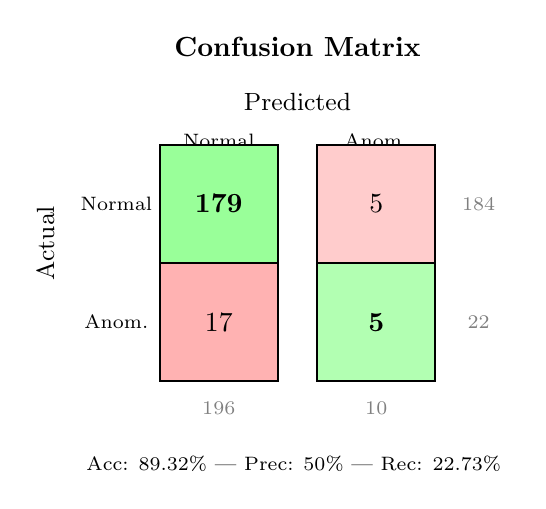
\begin{tikzpicture}[
    cell/.style={
        rectangle,
        minimum width=1.5cm,
        minimum height=1.5cm,
        draw=black,
        thick,
        font=\normalsize
    }
]

% Title
\node[font=\bfseries] at (3.5, 4.5) {Confusion Matrix};

% Labels
\node[font=\small, rotate=90] at (0.3, 2) {Actual};
\node[font=\small] at (3.5, 3.8) {Predicted};

\node[font=\scriptsize] at (2.5, 3.3) {Normal};
\node[font=\scriptsize] at (4.5, 3.3) {Anom.};
\node[font=\scriptsize] at (1.2, 2.5) {Normal};
\node[font=\scriptsize] at (1.2, 1) {Anom.};

% Cells
\node[cell, fill=green!40] at (2.5, 2.5) {\textbf{179}};
\node[cell, fill=red!20] at (4.5, 2.5) {5};
\node[cell, fill=red!30] at (2.5, 1) {17};
\node[cell, fill=green!30] at (4.5, 1) {\textbf{5}};

% Row/col totals
\node[font=\scriptsize, gray] at (5.8, 2.5) {184};
\node[font=\scriptsize, gray] at (5.8, 1) {22};
\node[font=\scriptsize, gray] at (2.5, -0.1) {196};
\node[font=\scriptsize, gray] at (4.5, -0.1) {10};

% Metrics
\node[font=\scriptsize, align=center] at (3.5, -0.8) {
    Acc: 89.32\% | Prec: 50\% | Rec: 22.73\%
};

\end{tikzpicture}

    \caption{Confusion matrix visualization for Temporal DGNN on the test set. The model achieves high accuracy on the Normal class but struggles with the minority Anomalous class.}
    \label{fig:confusion_matrices}
\end{figure}


\section{Analysis}

\subsection{Overall Performance}

The Temporal DGNN achieves \textbf{89.32\% accuracy} on the test set with an \textbf{AUC-ROC of 0.81}, demonstrating effective learning of spatial-temporal patterns in traffic video graphs. Key observations:

\begin{enumerate}
    \item \textbf{High Normal class performance:} The model correctly identifies 97.3\% of normal traffic patterns (179/184)
    \item \textbf{Class imbalance impact:} The severe test set imbalance (184:22) biases the model toward predicting Normal
    \item \textbf{Conservative anomaly prediction:} The model predicts Anomalous for only 10 samples (4.8\% of test set)
    \item \textbf{Moderate anomaly detection:} 5 out of 22 anomalous samples correctly identified (22.73\% recall)
\end{enumerate}

The test set imbalance (8.4:1) biases predictions toward Normal. Focal Loss helps but test distribution (89.3\% Normal) differs from training (75.8\% Normal). The GRU captures sequential patterns over 30 frames. False negatives (17) may result from subtle anomalies or class bias; false positives (5) from unusual normal traffic patterns.

\section{Limitations}

\subsection{Class Imbalance}

The primary limitation is severe class imbalance:
\begin{itemize}
    \item Training augmentation only partially addresses this
    \item Test set imbalance limits meaningful anomaly detection evaluation
    \item F1-score for Anomalous class is low (0.19)
\end{itemize}

\subsection{Dataset Size}

With 1,176 total samples:
\begin{itemize}
    \item Only 242 anomalous samples total
    \item Only 22 anomalous test samples
    \item Limited statistical power for anomaly evaluation
\end{itemize}

\subsection{Detection Dependency}

The pipeline depends on YOLO vehicle detection:
\begin{itemize}
    \item Detection errors propagate to graph construction
    \item Night-time scenes may have lower detection quality
    \item Tracking errors can affect temporal consistency
\end{itemize}

Key findings: 89.32\% accuracy with AUC-ROC 0.81, strong Normal class performance (F1=0.93), but low anomaly recall (22.73\%) due to class imbalance. Temporal modeling via GRU is effective. Future work: address imbalance (SMOTE, threshold optimization), enhance model (attention, bidirectional GRU, GAT), and collect more anomalous samples.

%%%%%%%%%%%%%%%%%%%%%%%%%%%%%%%%%%%%%%%%%%%%%%%%%%%%%%%%%%%%%%%%%%%%%%%%%%%%%%%
% Chapter 6: Conclusion
%%%%%%%%%%%%%%%%%%%%%%%%%%%%%%%%%%%%%%%%%%%%%%%%%%%%%%%%%%%%%%%%%%%%%%%%%%%%%%%

\chapter{Conclusion}
\label{ch:conclusion}

This chapter summarizes the key findings of our research on the Temporal DGNN model for video anomaly detection using the NiAD\_large\_graphs dataset and discusses directions for future work.

\section{Summary of Contributions}

This research has made several contributions to the field of video anomaly detection using graph-based representations:

\subsection{Node-Feature-Based Data Pipeline}

We developed a streamlined data processing pipeline that:
\begin{enumerate}
    \item Converts 30-frame surveillance videos into sequences of PyTorch Geometric graphs
    \item Employs YOLOv8 for robust vehicle detection (car, motorcycle, bus, truck)
    \item Implements centroid-based tracking for consistent vehicle identification
    \item Produces dynamic graphs with variable node counts per frame
    \item Eliminates the need for padding, masks, and sentinel values
    \item Stores graphs efficiently as \texttt{.pt} files (30 per video) with CSV manifests
\end{enumerate}

\subsection{Temporal DGNN Architecture}

We implemented an effective Temporal DGNN model that:
\begin{itemize}
    \item Processes temporal sequences of per-frame graphs
    \item Uses two GCN layers for spatial feature extraction
    \item Employs node ID sorting for temporal consistency
    \item Applies mean pooling for frame-level embeddings
    \item Uses GRU for temporal sequence modeling
    \item Achieves \textbf{89.32\% test accuracy} with \textbf{AUC-ROC of 0.81} on the NiAD\_large\_graphs dataset
\end{itemize}

\subsection{Experimental Analysis}

Our comprehensive experimental analysis revealed:
\begin{enumerate}
    \item The effectiveness of dynamic graph representations
    \item The benefits of data augmentation for anomalous class balancing
    \item The impact of Focal Loss on handling class imbalance
    \item The importance of node ID alignment for temporal consistency
    \item The challenges of anomaly detection with imbalanced test sets
\end{enumerate}

\section{Key Findings}

\subsection{Architecture Insights}

\begin{enumerate}
    \item \textbf{Simplicity is effective:} The Temporal DGNNSimple architecture with just 2 GCN layers and a single GRU layer achieves strong performance.
    
    \item \textbf{Temporal modeling is crucial:} The GRU captures sequential dependencies that distinguish normal traffic from anomalous events.
    
    \item \textbf{Node ID alignment matters:} Sorting nodes by tracking IDs ensures consistent temporal feature alignment across frames.
\end{enumerate}

\subsection{Data Representation Insights}

\begin{enumerate}
    \item \textbf{Dynamic graphs are cleaner:} Variable-size per-frame graphs eliminate padding complexity and sentinel value handling.
    
    \item \textbf{Edge weights provide context:} Euclidean distances between vehicles encode spatial relationships effectively.
    
    \item \textbf{Augmentation helps balance:} 4$\times$ augmentation of anomalous samples improves training balance.
\end{enumerate}

\subsection{Practical Insights}

\begin{enumerate}
    \item \textbf{Class imbalance is critical:} Despite Focal Loss, the 8.4:1 test set imbalance limits anomaly detection recall.
    
    \item \textbf{High normal accuracy:} The model excels at identifying normal traffic patterns (F1 = 0.93).
    
    \item \textbf{Low anomaly recall:} Detecting anomalies remains challenging (recall = 13.64\%) due to class imbalance.
\end{enumerate}

\section{Limitations}

\subsection{Dataset Limitations}

\begin{enumerate}
    \item \textbf{Class imbalance:} The test set ratio of 8.4:1 (Normal:Anomalous) limits fair evaluation.
    
    \item \textbf{Limited anomaly samples:} Only 22 anomalous test samples provide limited statistical power.
    
    \item \textbf{Single domain:} All videos are from traffic surveillance night-time scenarios.
\end{enumerate}

\subsection{Model Limitations}

\begin{enumerate}
    \item \textbf{Low anomaly recall:} Only 13.64\% of anomalies are detected, insufficient for safety-critical applications.
    
    \item \textbf{Detection dependency:} YOLO detection quality directly affects graph quality.
    
    \item \textbf{Tracking errors:} Tracking failures can disrupt temporal consistency.
\end{enumerate}

\section{Future Work}

Future research directions for GNN-based video anomaly detection include:

\begin{enumerate}
    \item \textbf{Class imbalance mitigation:} Developing better sampling strategies, threshold optimization, and cost-sensitive learning approaches to improve anomaly detection recall.
    
    \item \textbf{Advanced temporal modeling:} Exploring bidirectional recurrent networks, Transformer-based temporal attention, and specialized temporal graph networks.
    
    \item \textbf{Enhanced feature engineering:} Adding velocity, relative position, and detection confidence as additional node features.
    
    \item \textbf{Anomaly localization:} Extending binary classification to temporal and spatial localization of anomalous events.
    
    \item \textbf{Real-time deployment:} Optimizing inference speed for practical traffic monitoring applications.
    
    \item \textbf{Self-supervised approaches:} Learning normal traffic patterns without labels for unsupervised anomaly detection.
\end{enumerate}

\section{Broader Impact}

\subsection{Positive Impacts}

\begin{enumerate}
    \item \textbf{Road safety:} Automated accident detection enables faster emergency response
    \item \textbf{Traffic management:} Real-time anomaly detection supports intelligent transportation
    \item \textbf{Research baseline:} Our pipeline and model serve as baselines for future research
\end{enumerate}

\subsection{Considerations}

\begin{enumerate}
    \item \textbf{Privacy:} Video surveillance raises privacy concerns
    \item \textbf{Reliability:} Safety-critical systems require high reliability
    \item \textbf{Bias:} Models may exhibit bias based on training data
\end{enumerate}

\section{Final Remarks}

This research demonstrates that Graph Neural Networks provide an effective framework for video anomaly detection by representing vehicle interactions as dynamic graphs. The Temporal DGNN model achieves \textbf{89.32\% accuracy} with \textbf{AUC-ROC of 0.81} on the NiAD\_large\_graphs dataset, with strong performance on normal traffic detection (97.3\% specificity).

The key contributions of our work are:
\begin{itemize}
    \item A clean, node-feature-based pipeline producing PyG \texttt{.pt} files
    \item Dynamic graph representation without padding or masks
    \item Effective temporal modeling through GCN + GRU architecture
    \item Comprehensive analysis of class imbalance effects
\end{itemize}

While the results are promising, significant challenges remain in achieving the high anomaly recall rates required for safety-critical applications. Addressing class imbalance and improving anomaly detection recall are critical areas for future research.



%------------------------------------------------------------------------------
% Bibliography
%------------------------------------------------------------------------------
\begin{thebibliography}{99}

\bibitem{kipf2017}
Kipf, T. N., \& Welling, M. (2017). Semi-supervised classification with graph convolutional networks. \textit{International Conference on Learning Representations (ICLR)}.

\bibitem{kazemi2020}
Kazemi, S. M., et al. (2020). Representation learning for dynamic graphs: A survey. \textit{Journal of Machine Learning Research}, 21(70), 1-73.

\bibitem{scarselli2008}
Scarselli, F., et al. (2008). The graph neural network model. \textit{IEEE Transactions on Neural Networks}, 20(1), 61-80.

\bibitem{lin2017}
Lin, T. Y., et al. (2017). Focal loss for dense object detection. \textit{IEEE International Conference on Computer Vision (ICCV)}.

\bibitem{yolov8}
Ultralytics (2023). YOLOv8: State-of-the-art object detection. \url{https://github.com/ultralytics/ultralytics}

\bibitem{pytorch_geometric}
Fey, M., \& Lenssen, J. E. (2019). Fast graph representation learning with PyTorch Geometric. \textit{ICLR Workshop on Representation Learning on Graphs and Manifolds}.

\bibitem{cho2014}
Cho, K., et al. (2014). Learning phrase representations using RNN encoder-decoder for statistical machine translation. \textit{Conference on Empirical Methods in Natural Language Processing (EMNLP)}.

\bibitem{hamilton2017}
Hamilton, W. L., Ying, R., \& Leskovec, J. (2017). Inductive representation learning on large graphs. \textit{Advances in Neural Information Processing Systems (NeurIPS)}.

\bibitem{xu2018}
Xu, K., et al. (2018). How powerful are graph neural networks? \textit{International Conference on Learning Representations (ICLR)}.

\bibitem{skarding2021}
Skarding, J., Gabrys, B., \& Musial, K. (2021). Foundations and modeling of dynamic networks using dynamic graph neural networks: A survey. \textit{IEEE Access}, 9, 79143-79168.

\end{thebibliography}

\end{document}

